\documentclass{standalone}

\def\pgfsysdriver{pgfsys-dvisvgm.def}
\usepackage{xcolor,lmodern,tikz}

\usetikzlibrary{arrows.meta,bending,scopes}

\begin{document}
\nopagecolor
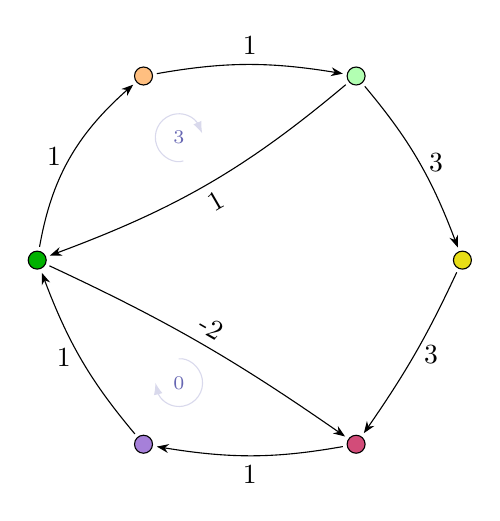
\begin{tikzpicture}
    [obj/.style={circle, minimum size=6.5pt, inner sep=1pt, draw=black},
    morph/.style={-{Stealth[length=1.5mm]}, thin, shorten >= 0.5mm, shorten <= 0.5mm},
    loop/.style={-{Latex[length=1.5mm]}, draw=blue!50!black!15, shorten >= 0.5mm, shorten <= 0.5mm}]
    \newdimen\R
    \R=2.7cm
    % Vertices
    \node[obj, fill=green!30       ] (A) at ( 60:\R) {};
    \node[obj, fill=orange!50      ] (B) at (120:\R) {};
    \node[obj, fill=green!70!black ] (C) at (180:\R) {};
    \node[obj, fill=red!30!blue!50 ] (D) at (240:\R) {};
    \node[obj, fill=purple!70      ] (E) at (300:\R) {};
    \node[obj, fill=yellow!90!black] (F) at (360:\R) {};

    % Edges
    \draw[morph] (A) edge[bend left=10] node[right] {3} (F);
    \draw[morph] (F) edge[bend left=5] node[right] {3} (E);
    \draw[morph] (E) edge[bend left=10] node[below] {1} (D);
    \draw[morph] (D) edge[bend left=10] node[left]  {1} (C);
    \draw[morph] (C) edge[bend left=20] node[left]  {1} (B);
    \draw[morph] (A) edge[bend left=10] node[below, sloped] {1}  (C);
    \draw[morph] (B) edge[bend left=10] node[above] {$1$} (A);
    \draw[morph] (C) edge[bend left=5] node[above, sloped] {-2} (E);

    % Faces
    \draw[loop] (barycentric cs:A=1,B=1,C=1) node[thin, blue!50!black!60, font=\fontsize{7}{0}\selectfont] {3} ++(290:.3) arc (290:0:.3);
    \draw[loop] (barycentric cs:C=1,D=1,E=1) node[thin, blue!50!black!60, font=\fontsize{7}{0}\selectfont] {0} ++(100:.3) arc (100:-190:.3);
 \end{tikzpicture}
\end{document}
